\documentclass[fleqn]{jbook}
\usepackage{physpub}
\newcommand{\md}{\mathrm{d}}

% amsmath, graphicx は自動的に読み込まれるので
% \usepackage しないでください、してもかまわないけど。
\begin{document}

\begin{question}{問題6}{榎戸輝揚・竹内一将}
液体ヘリウムの密度は、図1のように平行平板コンデンサーとコイルを並列につないだLC回路を作り、コンデンサーの間隙を液体ヘリウムで満たしてコンデンサーの容量を測定し、求めることができる。\par
ヘリウムの分極率を$\alpha$とすると、密度$\rho$と比誘電率$\epsilon$の間には次の式が成り立つ。ただし、$k$は比例定数である。
また、$\epsilon$は真空中の誘電率$\epsilon_0$に対する誘電率の比であり、無次元の量である。
\[
\frac{1}{k}\alpha \rho=\frac{\epsilon -1}{\epsilon +2 }
\]
ヘリウムの分極率は温度と圧力にほとんど依存しないことが知られているため、この実験方法は、密度の温度依存性、圧力依存性などを調べるときに用いられる。以下の設問に答えよ。

% 図の挿入
\begin{figure}[htbp]
  \begin{center}
    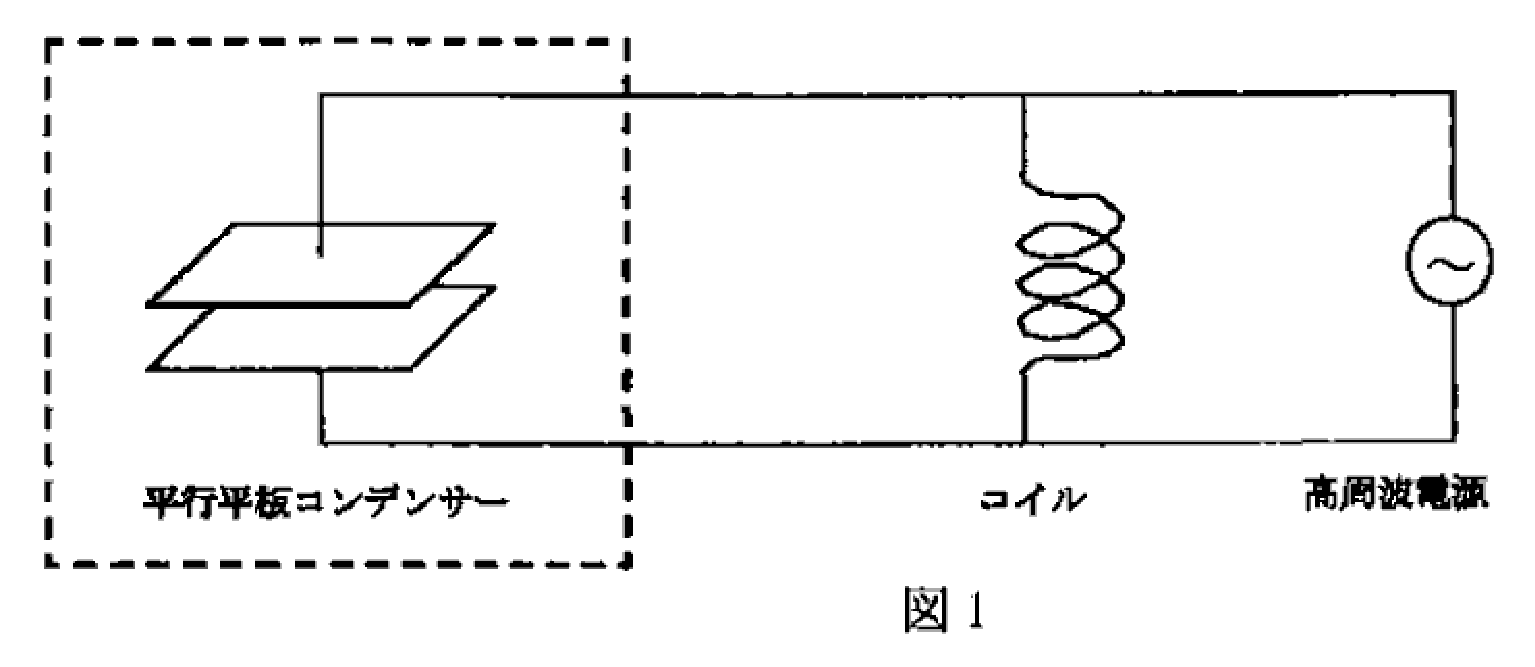
\includegraphics[width=110mm]{2003phy6-1.eps}
  \end{center}
  %\caption{図1}%{}内にタイトルを記入してください
  \ilabel{fig:2003phy6-1.eps}
\end{figure}

\begin{enumerate}
\item 図1のLC回路において、平行平板コンデンサーの間隙が真空のときの容量を$C_0$、コイルのインダクタンスを$L$として共振振動数($f_0$)を求めよ。回路の抵抗、浮遊容量は考えなくてよい。
\item 室温で図1のLC回路の$f_0$を測定したところ10MHzとなった。このとき、コイルのインダクタンスは10$\mu$H、コンデンサーの平行平板の面積は$1.0\times 10^{-4}\mathrm{m}^2$であった。コンデンサーの間隙はいくらか。コンデンサーの間隙は真空とし、真空の誘電率($\epsilon_0$)を$8.9\times10^{-12}\mathrm{F/m}$として求めよ。
\item コンデンサーの間隙を真空に保ったまま、図1の点線で囲まれた部分の温度を下げて共振振動数を測定したところ、温度の低下と共に共振振動数が変化した。考えられる原因について述べよ。
\item コンデンサーの間隙を液体ヘリウム(密度$\rho$)で満たしたときの共振振動数($f$)を$\rho$の関数で表わし、4.2Kの液体ヘリウム($\rho=1.3\times10^2 \mathrm{kg/m^3}$)で満たしたときの共振振動数を求めよ。$\alpha/k=1.1\times 10^{-5}\mathrm{m^3/kg}$である。
\item 共振振動数の測定精度が1Hzのとき、液体ヘリウムの密度の測定精度がいくらになるか述べよ。

% 図の挿入
\begin{figure}[htbp]
  \begin{center}
    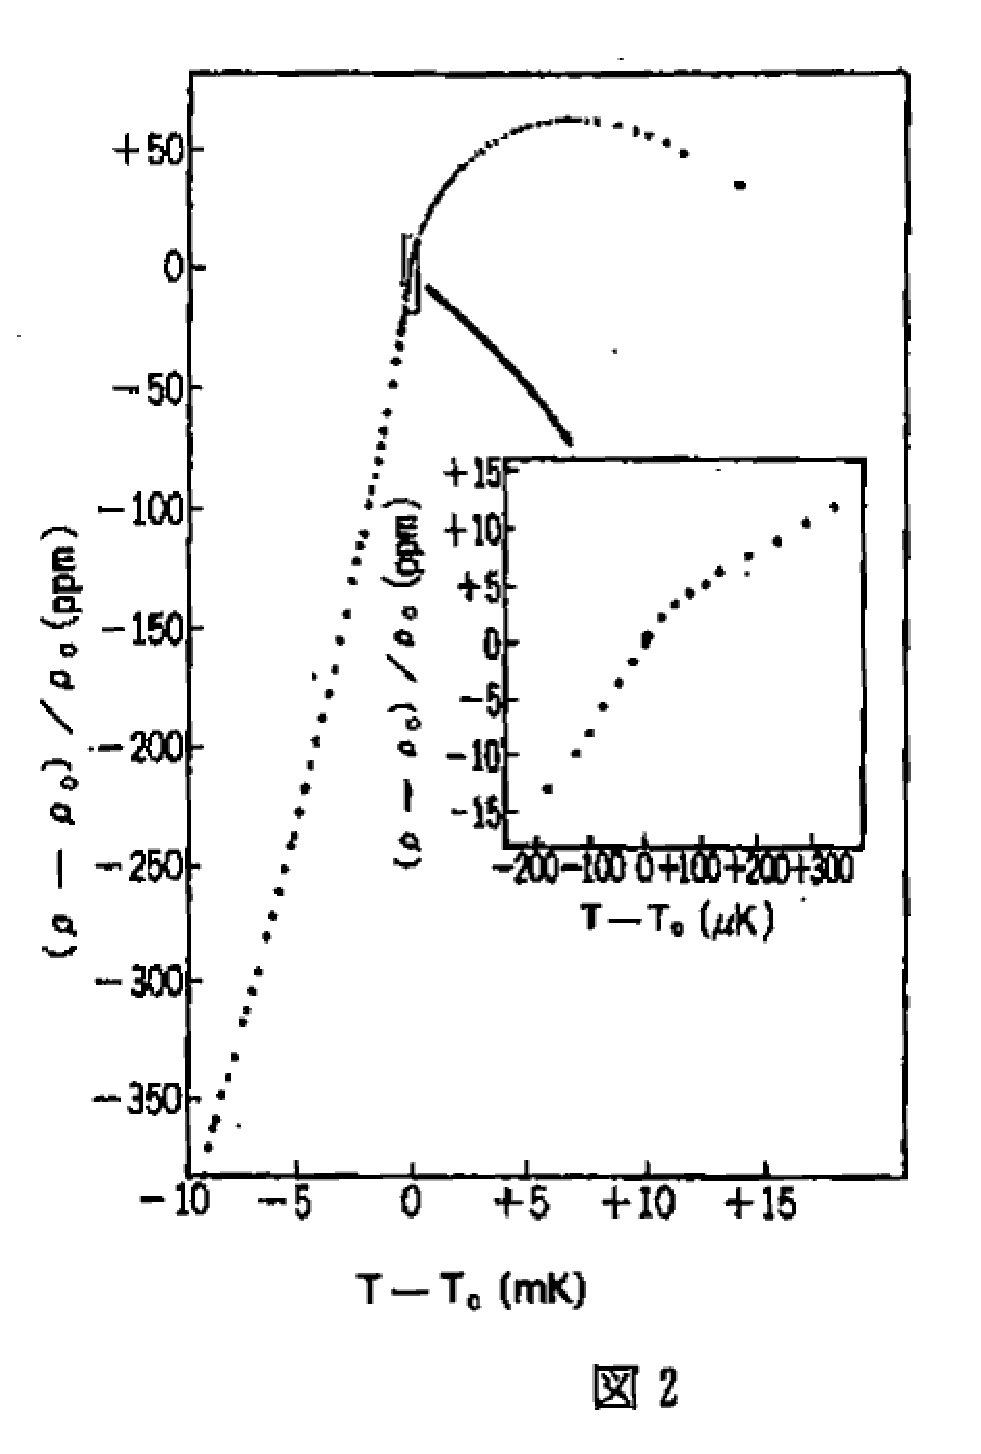
\includegraphics[width=80mm]{2003phy6-2.eps}
  \end{center}
  %\caption{図2}%{}内にタイトルを記入してください
  \ilabel{fig:2003phy6-2.eps}
\end{figure}

\item 図2は、この方法を使って、液体ヘリウムの密度$\rho$をある温度$T_0(2.2\mathrm{K})$の近傍で測定し、$T_0$での密度$\rho_0$に対する相対値を表わしたものである。この図をもとに、温度$T_0$付近での液体ヘリウムの密度の温度依存性の特徴とその原因について述べよ。
\item 低温実験では、白金、炭素、ゲルマニウムなどの抵抗値を測定して2次温度計として利用することが多い。図3は、白金抵抗温度計と炭素抵抗温度計の抵抗値の温度依存性を示したものである。図2に示した液体ヘリウムの密度の温度依存性の測定には、どちらの温度計を用いるのが適当か、その理由と共に述べよ。
\item 図3からわかるように、白金抵抗温度計の抵抗値が温度の増加と共に大きくなるのに対し、炭素抵抗温度計の抵抗値は温度の増加と共に小さくなる。それぞれの抵抗温度計の抵抗値が示す温度依存性の原因を述べよ。
\end{enumerate}

% 図の挿入
\begin{figure}[htbp]
  \begin{center}
    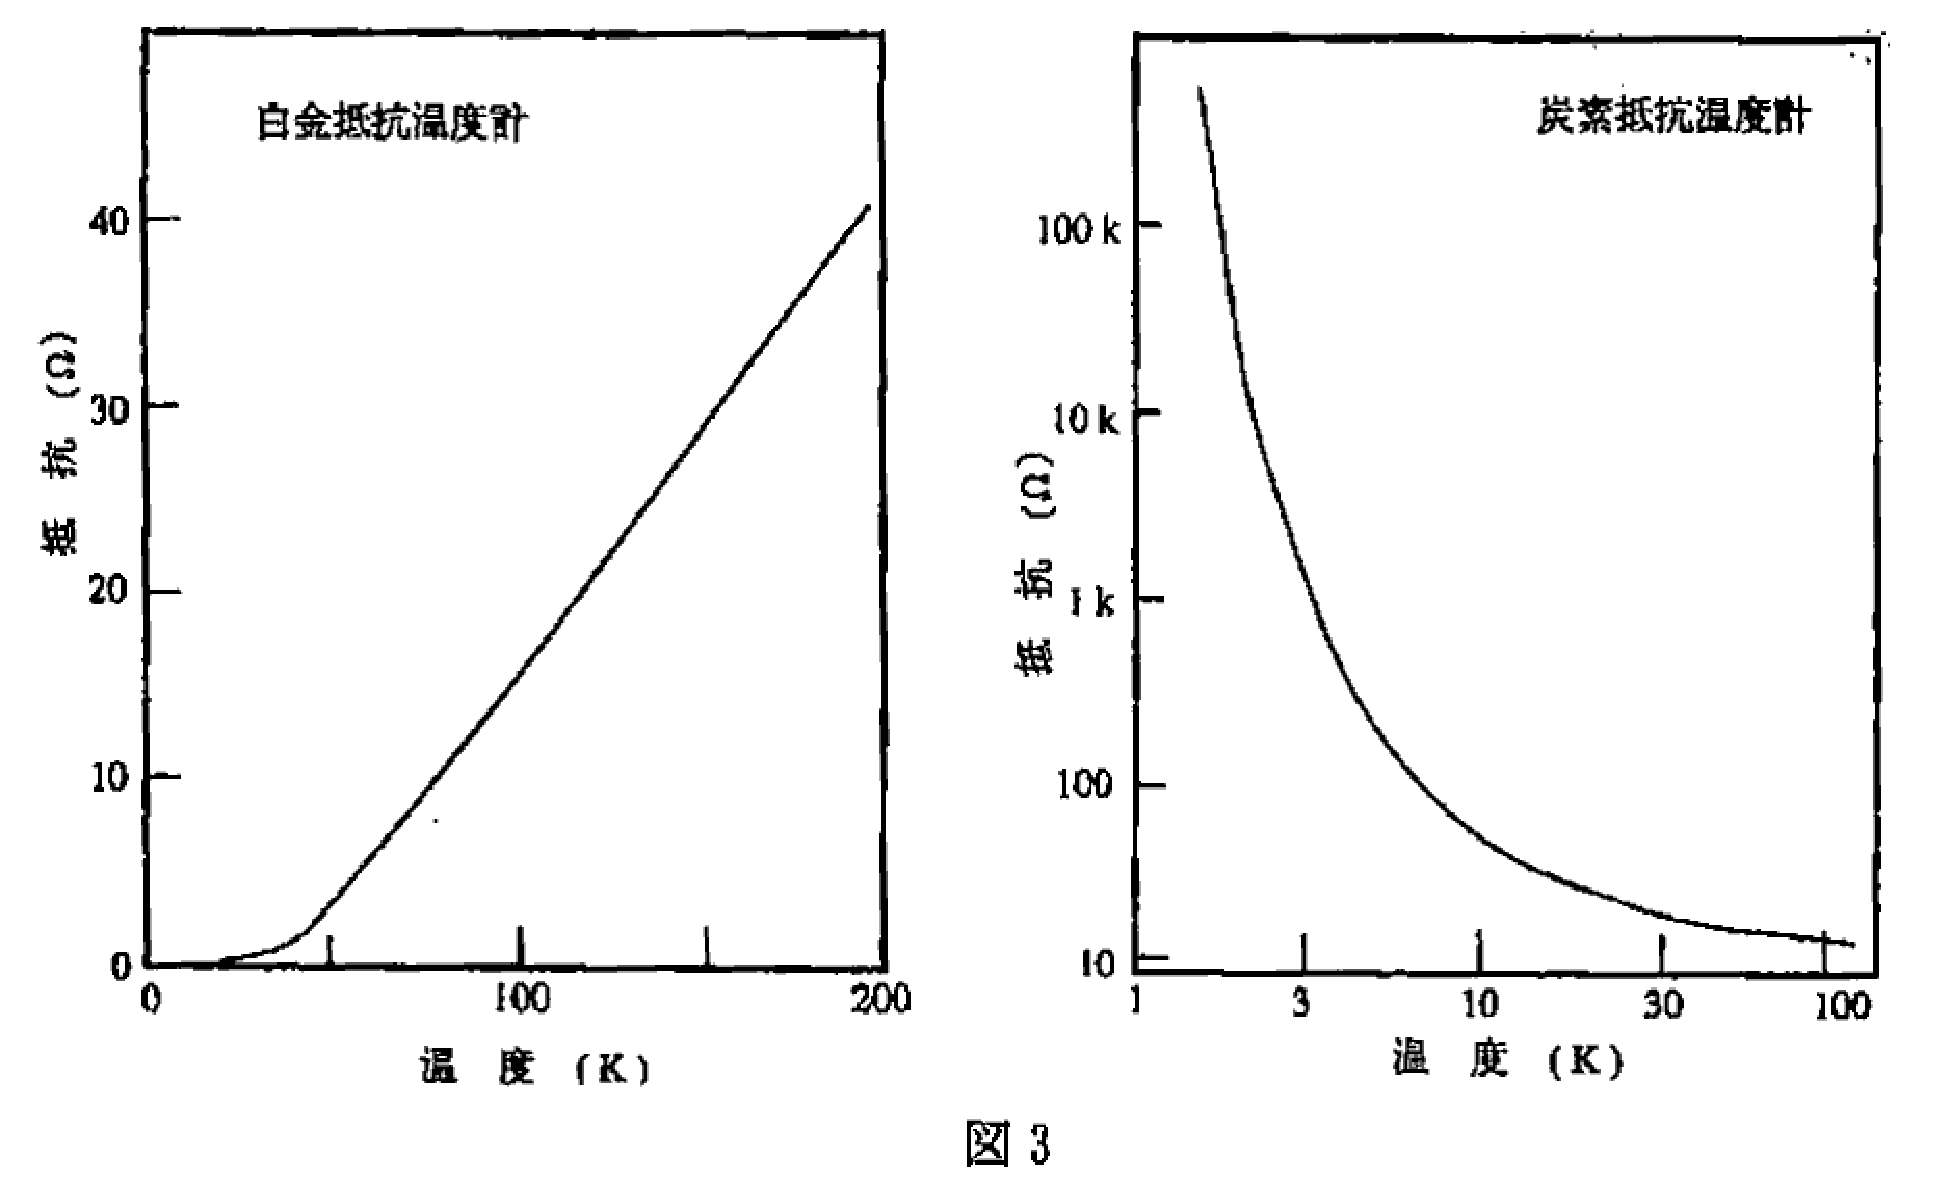
\includegraphics[width=150mm]{2003phy6-3.eps}
  \end{center}
  %\caption{図3}%{}内にタイトルを記入してください
  \ilabel{fig:2003phy6-3.eps}
\end{figure}

\end{question}

%2003phy4-1.ep

\begin{answer}{問題6}{榎戸輝揚・竹内一将}
\begin{enumerate}
\item キルヒホッフの法則を閉回路に適用した$\frac{1}{C_0}\int I \md t+L \frac{\md I}{\md t}=0$
において$I\propto e^{i\omega _0 t}(\omega_0:\text{共振角周波数})$を代入すると、
\begin{eqnarray*}
\frac{I}{iC_0\omega _0}+i\omega_0 LI&=&0  \\
\omega_0&=&\frac{1}{\sqrt{LC_0}} \\
\end{eqnarray*}
したがって、求める共振振動数は
\begin{eqnarray}
\ilabel{kyoumei}
f_0=\frac{\omega_0}{2\pi}=\frac{1}{2\pi \sqrt{LC_0}}   
\end{eqnarray}
である。

\item コンデンサーの容量$C_0$は、平板の面積を$S$、間隙の長さを$d$とすると、
\begin{eqnarray}
 \ilabel{youryou}
C_0=\epsilon_0\frac{S}{d}  
\end{eqnarray}
であるから、式(\iref{kyoumei})(\iref{youryou})より、
\[
d=\epsilon_0LS(2\pi f_0)^2
\]
ここへ$f_0=10[\mathrm{MHz}] \ ,L=10[\mathrm{\mu H}] \ , S=1.0\times 10^{-4}[ \mathrm{m^2}]$を代入すると、
\[
d=3.5\times 10^{-5}[\mathrm{m}]=35[\mathrm{\mu m}]
\]

\item 温度が下がると、コンデンサーの平板が熱収縮して式(\iref{youryou})の$S$が減少する。これによって$C_0$が小さくなり、共振振動数$f_0$は上昇する。\par
(注)なお、平板間を支えている支柱が収縮することで$d$も減少することが考えられるが、式(\iref{youryou})の分子の$S$は面積の次元を持つのに対して、分母の$d$は距離の次元であるから、分子がより強く効いて$C_0$は減少するだろう。

\item 
コンデンサーの間隙を液体ヘリウムで満たしたときの容量は、比誘電率$\epsilon$を用いて、
\begin{eqnarray}
C=\epsilon \epsilon_0 \frac{S}{d}=\epsilon C_0
\ilabel{youryou2}
\end{eqnarray}
と書ける。また問題で与えられた式
\[
\frac{\alpha}{k}\rho=\frac{\epsilon-1}{\epsilon +2}
\]
を$\epsilon$について解くと、
\begin{eqnarray}
\epsilon=\frac{1+2\alpha \rho/k}{1-\alpha \rho/k}
\ilabel{epsilon}
\end{eqnarray}
である。この2式(\iref{youryou2})(\iref{epsilon})を用いると、共振振動数は次のように書ける。
\begin{eqnarray}
f=\frac{1}{2\pi \sqrt{LC}}=\frac{f_0}{\sqrt{\epsilon}}=\sqrt{\frac{1-\alpha \rho/k}{1+2\alpha \rho/k}}f_0
\ilabel{f}
\end{eqnarray}
いま、
\[
\frac{\alpha}{k}\rho=1.43\times 10^{-3} \ll 1
\]
であるから、$\alpha \rho/k$の2次以上の項を無視すれば、次のように近似できる。
\begin{eqnarray}
f &\simeq& \left(1-\frac{1}{2}\frac{\alpha \rho}{k}\right) \left(1-\frac{\alpha \rho}{k} \right)f_0 \nonumber\\
& \simeq & (1-\frac{3}{2}\frac{\alpha \rho}{k})f_0 \ilabel{kinnzi}\\
&=&9.979[\mathrm{MHz}] \nonumber %9.978としてもよいかも%
\end{eqnarray}


\item 
測定精度$\triangle f=1[\mathrm{Hz}]$のとき、共振振動数$f$と$f+\triangle f$とを識別できるとする。
これに対応して、液体ヘリウムの密度を$\rho$、$\rho - \triangle \rho$とすると、
$\alpha \rho/k$が1に対して十分に小さい範囲では、式(\iref{kinnzi})が使えるから、
\begin{eqnarray*}
\frac{f}{f_0}&\simeq& 1-\frac{3}{2}\frac{\alpha \rho}{k}\\
\frac{f+\triangle f}{f_0}&\simeq& 1-\frac{3}{2}\frac{\alpha (\rho-\triangle \rho)}{k}
\end{eqnarray*}
辺々を引くことで、
\[
\triangle \rho=\frac{2}{3}\frac{k}{\alpha}\frac{\triangle f}{f_0}=6\times 10^{-3}[\mathrm{kg/m^3}]=6[\mathrm{g/m^3}]
\]
が密度の測定精度となる。\par

\item
$T_0$より高い温度では、通常の液体に多く見られるように温度が高くなるにしたがって密度が低くなる性質があるのに対し、
$T=T_0$以下では温度の上昇にともなって密度が上昇している。また、$T=T_0$では密度にカスプが見られる。\par

密度$\rho$はギブスの自由エネルギー$G$と$\rho \propto \frac{N}{V} \propto \frac{1}{\frac{\partial G}{\partial p}}$の関係にあり、
$T=T_0$に密度のカスプがあることから、ギブス自由エネルギーは1階微分にカスプがあり、$T_0$に2次相転移点を持つことが予想される。
実際、液体ヘリウム$^4\mathrm{He}$は$T_0=2.2[\mathrm{K}]$が$\lambda$点と呼ばれる2次の相転移点であることが知られており、
これを境にして高温側は$\mathrm{He}$I と呼ばれる常流動相、低温側は$\mathrm{He}$II と呼ばれる超流動相であるので、これが密度の温度依存性の由来であると考えられる。

\item
図2での液体ヘリウムの測定温度は2.2[K]前後であるから、この範囲で温度に対する抵抗の変化が大きい炭素抵抗温度計の方が測定に適していると考えられる。

\item
(白金抵抗温度計)白金の格子結晶を構成する原子は、その平衡位置付近で格子振動を行う。この格子振動が格子配列の周期性を乱し、結晶内を移動する電子と電子−格子相互作用を起こすことで電気抵抗の原因となっている。高温では格子振動の影響が強く効くため、電気抵抗が大きくなる。\par
(炭素抵抗温度計)炭素抵抗温度計は半導体としての性質を持つと考えられる。価電子帯から伝導体へバンドギャップを超えて電子が励起されると、伝導体の伝導電子と価電子帯のホールの両方が電気伝導を担うキャリアとなる。温度が高くなると、この励起される電子の数が増加してキャリアが増えるために電気抵抗は減少する。


\end{enumerate}
\end{answer}


\end{document}
